\chapter{基于模型的方法计算$\CTL$下的遗忘}\label{chapter05}

{\em
	遗忘与均匀插值是一对对偶概念,已有研究表明$\CTL$不具有均匀插值性质~\cite{Maksimova:JANCL:1991},这就表明$\CTL$中的遗忘理论不是封闭的\footnote{对于给定的逻辑语言${\cal L}$和该语言上的操作${\cal O}$,若$\cal O$作用到$\cal L$中的元素后得到的结果仍然在$\cal L$中,则称$\cal O$在$\cal L$下是封闭的。}。
	此时,探索$\CTL$下遗忘理论封闭的情形对深入引用遗忘理论有重要意义。
	为此,本章首先提出有限初始$\MPK$-结构的特征公式;其次,表明$\CTL$公式的遗忘结果在此情形下可以表示成其模型的特征公式的吸取;最后,提出一种基于模型的方法计算遗忘,且探索了如何使用遗忘计算最弱充分条件和知识更新。
}

\section{引言}\label{sec:chapter06_introduction}
%系统模型通常是有限的
%小模型理论,公式的长度有限
%描述数(特征数)来区分同意结构内那些状态在一定程度上是相同的,如果超过这个度,肯定不同。此时,就可以使用CTL公式来描述这些状态及其关系。
%描述forgetting的四个规则。

计算树逻辑是由Clarke和Emerson提出的一种分支时间时序逻辑,它能很好的描述并发系统的一些性质,包括:互斥属性和安全属性等。
Emerson和Halpern证明$\CTL$具有小模型属性:如果一个公式是可满足的,那么它在一个小的有限模型下是可满足的~\cite{DBLP:journals/jcss/EmersonH85}。
具体说来,对于给定的$\CTL$公式$\varphi$,如果公式的长度\footnote{给定公式$\varphi$,出现在该公式里的符号的个数为公式的长度,记为$|\varphi|$。}为$n$(记为:$|\varphi| = n$),则存在一个状态数为$n8^n$的初始结构$(\Hm,s_0)$使得$(\Hm,s_0)\models \varphi$。

此外,现实情况下能处理的系统都是有限的,且在某一固定环境下所涉及到的原子命题是有限的。因此,在这部分讨论一种约束的$\CTL$,即:(1)出现在$\CTL$公式中的原子命题的个数是有限的(即$\Ha$是有限的);(2)初始结构的状态空间$S$是一个有限的固定状态空间${\cal S}=\{b_1,\ldots,b_m\}$的子集(即$S \subseteq {\cal S}$),且使得对于任意约束长度的$\CTL$公式$\varphi$,若$\varphi$是可满足的,则存在一个初始结构$(\Hm,s_0)$使得$(\Hm,s_0)\models \varphi$且其状态空间是${\cal S}$的子集。由此可见,在这种情形下只有有限个初始结构应该被考虑。
下文将表明在这一约束条件下$\CTL$中的遗忘是封闭的。

本章其余部分组织如下:首先,第\ref{chapter06:sec:des}节定义一种约束$V$-互模拟的概念,然后给出初始结构的特征公式。其次,第\ref{chapter06:sec:close}节描述约束$\CTL$下的遗忘是封闭的,并给出计算方法。进一步,第\ref{chapter06:sec:algm}节给出基于模型的计算遗忘的算法,并分析算法的复杂性。最后,进行本章工作总结。

\section{描述初始结构}\label{chapter06:sec:des}%\label{sec:chapter06_chaIntC}
本节介绍与一个初始结构相关的$\CTL$公式——特征公式是如何得到的。
%对于一个给定的有限初始结构(状态个数和$\Ha$都是有限的),其不循环的计算树(状态不重复出现)的深度最多为其状态数的个数。
对于一个给定的初始结构,其特征公式与其计算树的特征公式密切相关。
为此,本节首先介绍计算树之间的$V$-互模拟关系,然后给出计算树的特征公式的定义,最后给出初始结构的特征公式。

\subsection{计算树的$V$-互模拟}
在第\ref{chapter03}章中的定义~\ref{def:VInd:bisimulation}给出了$\Ind$-结构($(\Hm,s_0)$中的$\Hm$为初始$\Ind$-Kripke结构)之间的$V$-互模拟定义及其相关性质,结构($(\Hm,s_0)$中的$\Hm$为初始Kripke结构)之间的$V$-互模拟有相同的定义,且不难证明$\Ind$-结构之间$V$-互模拟有的性质结构之间$V$-互模拟也有。此外,第\ref{chapter03}章遗忘有的性质在本章的约束情形下也有,这里不再赘述。本节给出结构之间的$V$-互模拟在有限结构下与下面将要给出的约束$V$-互模拟等价——与深度$n$关联的$V$-互模拟。但是为了方便,本章仍然引入约束$V$-互模拟的概念。

首先给出能够描述一定深度$n\in \mathbb{N}$的计算树之间的$V$-互模拟关系,记为$\Hb_n^V$。令$V\subseteq \Ha$是原子命题的集合,$i\in \{1,2\}$,$\Hm_i=(S_i,R_i,L_i,s_0^i)$是初始Kripke结构,${\cal K}_i=(\Hm_i, s_i)$是结构。$\Hb_n^V$被递归定义如下:
\begin{itemize}
	\item 若$L_1(s_1)-V=L_2(s_2)$,则$({\cal K}_1,{\cal K}_2) \in \Hb_0^V$;
	\item 对任意$n\ge 0$,若满足下面几个条件,则$({\cal K}_1,{\cal K}_2)\in \Hb_{n+1}^V$成立:
	\begin{itemize}
		\item $({\cal K}_1,{\cal K}_2) \in \Hb_0^V$;
		\item 对任意$(s_1,s_1')\in R_1$,存在$(s_2,s_2')\in R_2$使得$({\cal K}_1',{\cal K}_2') \in \Hb_n^V$;
		\item 对任意$(s_2,s_2')\in R_2$,存在$(s_1,s_1')\in R_1$使得$({\cal K}_1',{\cal K}_2') \in \Hb_n^V$。
	\end{itemize}
\end{itemize}
其中${\cal K}_i'=(\Hm_i,s_i')$。

当所谈及的原子命题的集合$V$很显然的时候,上述$\Hb_n^V$中的$V$可以省略,记为$\Hb_n$。此外,当讨论的$\Hm_i$$(i=1,2)$是显然的时候,可以使用$(s_1,s_2) \in \Hb_n$代替$((\Hm_1,s_1),(\Hm_2,s_2)) \in \Hb_n$。
此时,约束$V$-互模拟关系就可以定义如下:
\begin{definition}[约束$V$-互模拟]\label{def:V-bisimulation}
	令$V$是$\Ha$的一个子集,$i\in \{1,2\}$, ${\cal K}_1$和${\cal K}_2$是结构。
	\begin{itemize}
		\item ${\cal K}_1$和${\cal K}_2$是约束$V$-互模拟的,当且仅当对所有的$n \ge 0$都有$({\cal K}_1, {\cal K}_2)\in \Hb_n$。若${\cal K}_1$和${\cal K}_2$是约束$V$-互模拟的,则记为${\cal K}_1 \overset{B}{\lrto}_V {\cal K}_2$。
		\item 对$\Hm_i$上的路径$\pi_i=(s_{i,1},s_{i,2},\dots)$,若对于任意的$j\in \mathbb{N}_{\ge 1}$\footnote{$\mathbb{N}$为整数的集合,$\mathbb{N}_{\ge 1}$是大于等于1的整数的集合。}都有${\cal K}_{1,j} \overset{B}{\lrto}_V {\cal K}_{2,j}$,则$\pi_1 \overset{B}{\lrto}_V \pi_2$。其中${\cal K}_{i, j}=(\Hm_i, s_{i,j})$。
	\end{itemize}
\end{definition}

值得注意的是,满足约束$V$-互模拟关系的结构之间有且仅有一个约束$V$-互模拟关系,即$\Hb_{k+1} = \Hb_k$ ($k \in \mathbb{N}$)。
%上述约束$V$-互模拟的定义是现有互模拟定义的一般化,这可以从下面几个方面来体现\footnote{在其他领域也有类似的定义,如:定义在数据库相关文献中的概念$k$-互模拟\cite{kaushik2002updates}。$k$-互模拟概念中涉及与本文$\Hb_n$类似的定义,只是其关系是从相反的方向(即:从孩子到父节点的方向)来说明的。此外,值得一提的是,本文的$V$-互模拟的概念是定义在$\MPK$-结构上的。}。
%首先,当给定的$V$为空集且谈论指定的初始状态时,本文的$V$-互模拟与定义在Baier等文章里的互模拟等价(定义7.1\cite{Baier:PMC:2008})的概念一致。
%其次,在上述文章里的基于状态的互模拟(定义7.7\cite{Baier:PMC:2008})是定义在给定结构的状态上的,因此与本文的$V$-互模拟(定义在结构的集合上)也不同。
%最后,本文的$\Hb_n$的定义与Browne的论文中的状态等价$E_n$类似,只是后者是定义在状态上\cite{browne1988characterizing}而本文的定义在$\MPK$-结构(或$\Ind$-结构)上。


\begin{lemma} \label{lem:HbBis}
	对于有限初始Kripke结构,约束 $V$-互模拟是一个 $V$-互模拟。
	%Let $V \subseteq \Ha$ and ${\cal K}_i=({\cal M}_i,s_i)~(i\in\{1,2\})$ and $\Hm_i=(S_i, R_i,L_i, s_0^i)$ be finite initial structures. 
	%Then every bounded $V$-bisimulation is a $V$-bisimulation between $\Hm_1$ and $\Hm_2$.
	%If $s_1 \lrto_V s_2$, then the bounded $V$-bisimulation {\cal B}_V containing $(s_1, s_2)$ is also a $V$-bisimulation (containing $(s_1,s_2)$) between $\Hm_1$ and $\Hm_2$.
\end{lemma}

\begin{proof}
	令 $V \subseteq \Ha$、 ${\cal K}_i=({\cal M}_i,s_i)~(i\in\{1,2\})$ 和 $\Hm_i=(S_i, R_i,L_i, s_0^i)$ 为有限的初始-Kripke 结构。
	因为$S_i~(i=1,2)$是有限的,所以$\Hb_n\subseteq S_1\times S_2~(n\ge 0)$ 都是有限的。
	由于对任意的$n\geq 0$都有 $\Hb_{n+1} \subseteq \Hb_n$。
	因此,存在一个最小数$k$使得
	$\Hb_{k+1} =\Hb_k$ (用 $\Hb$表示)。

	
	这里证明对任意的 $r_1\in S_1$ 和 $r_2 \in S_2$,有 $(r_1, r_2)\in \Hb$ 蕴涵 %if and only if
	\begin{itemize}
		\item[(a)] $L_1(r_1)-V = L_2(r_2)-V$;
		\item[(b)] $\forall w_1\in S_1$,若$(r_1, w_1)\in R_1$,则 $\exists w_2 \in S_2$ 使得 $(r_2,w_2) \in R_2$ 和 $(w_1, w_2) \in \Hb$; 和
		\item[(c)] $\forall w_2\in S_2$,若$(r_2, w_2)\in R_2$,则 $\exists w_1 \in S_1$ 使得 $(r_1,w_1) \in R_1$ 和 $(w_1, w_2)\in \Hb $。
	\end{itemize}
	
	首先,由对任意的$n\ge 0$都有$(r_1, r_2)\in \Hb_n$可知 $(r_1, r_2) \in \Hb_0$,这意味着
	$L_1(r_1)-V = L_2(r_2)-V$。因此(a)成立。
	
	其次,令$w_1 \in S_1$ 和 $(r_1, w_1)\in R_1$。有 \\
	$(r_1,r_2)\in \Hb$、 $w_1 \in S_1$ 和 $(r_1, w_1)\in R_1$\\
	$\Rto$ 由$\Hb_{k+1}=\Hb$知$(r_1,r_2)\in \Hb_{k+1}$、 $w_1 \in S_1$ 和 $(r_1, w_1)\in R_1$\\
	$\Rto$ 由定义可知$\exists w_2\in S_2$使得 $(r_2, w_2)\in R_2$ 和 $(w_1,w_2)\in \Hb_k$\\
	$\Rto$ 由$\Hb=\Hb_k$可知$\exists w_2\in S_2$ 使得 $(r_2, w_2)\in R_2$ 和 $(w_1,w_2)\in \Hb$\\
	$\Rto$ (b)成立。
	
	可以类似地证明 (c)也成立。
	因此, $\Hb$ 是$\Hm_1$ 和 $\Hm_2$之间的一个 $V$-互模拟关系。
\end{proof}

由引理~\ref{lem:HbBis}可知,$\Hb$既是一个约束$V$-互模拟关系也是一个$V$-互模拟关系,因此下面的推论是显然成立的。
\begin{corollary} \label{lem:bounedToGe}
	令 $V \subseteq \Ha$ 和 ${\cal K}_i=({\cal M}_i,s_i)$ ( $i\in\{1,2\}$),其中 $\Hm_i=(S_i, R_i,L_i, s_0^i)$ 是有限的初始Kripke结构。则
	%$s_1 \overset{\Hb}{\lrto}_V s_2$ 
	$s_1$ 和 $s_2$ 是约束 $V$-互模拟的当且仅当$s_1 \lrto_V s_2$。
\end{corollary}

%\begin{lemma}
%给定原子命题集合$V\subseteq \Ha$和$\MPK$-结构,其中$i=1,2$且$\Hm_i=(S_i, R_i, L_i, s_0^i)$为有限初始结构。$(s_1, s_2)\in \Hb$当且仅当$s_1 \lrto_V s_2$。
%\end{lemma}
%\begin{proof}
%	%由于$\Hb$是${\cal K}_1$和${\cal K}_2$的约束互模拟关系,所以$(s_1, s_2)\in \Hb$。
%	值得注意的是对任意的$n\geq 0$,都有$\Hb_{n+1} \subseteq \Hb_n$。又因为$\Hb_0\subseteq S_1 \times S_2$ 是有限的,因而存在一个数$k$使得$\Hb_{k+1}=\Hb_k = \Hb$。
%	
%	(1)证明若$(s_1, s_2)\in \Hb$则$s_1 \lrto_V s_2$。
%	显然,$(s_1, s_2)\in \Hb$。所以,只需要证明$\Hb$是$\Hm_1$和$\Hm_1$之间的一个$V$-互模拟关系。
%	下面证明对任意的$r_1\in S_1$和$r_2\in S_2$,$(r_1,r_2) \in \Hb$当且仅当
%	\begin{itemize}
%		\item[(a)] $L_1(r_1)-V = L_2(r_2)-V$;
%		\item[(b)] $\forall w_1\in S_1$, 若 $(r_1, w_1)\in R_1$,则 $\exists w_2 \in S_2$ 使得 $(r_2,w_2) \in R_2$ 和 $(w_1, w_2) \in \Hb$;和 
%		\item[(c)] $\forall w_2\in S_2$,若 $(r_2, w_2)\in R_2$,则 $\exists w_1 \in S_1$ 使得 $(r_1,w_1) \in R_1$ 和 $(w_1, w_2)\in \Hb $。
%	\end{itemize}
%
%	$(\Rto)$ $(r_1,r_2) \in \Hb$\\
%	$\Rto$ $\forall n\geq 0$,$(r_1,r_2)\in \Hb_n$\\
%	$\Rto$ $(r_1,r_2)\in \Hb_0$且$\forall n > 0$,$(r_1,r_2)\in \Hb_n$\\
%	$\Rto$ $L_1(r_1)-V = L_2(r_2)-V$ (因此,(a)成立),
%	
%	且$\forall n\geq 0$,$(r_1,r_2)\in \Hb_{n+1}$意味着下面几点成立:
%	\begin{itemize}
%		\item $L_1(r_1)-V = L_2(r_2)-V$;
%		\item $\forall w_1 \in S_1$,若$(r_1, w_1)\in R_1$,则$\exists w_2 \in S_2$使得$(r_2,w_2) \in R_2$且$(w_1, w_2) \in \Hb_n$;且
%		\item $\forall w_2\in S_2$,若$(r_2, w_2)\in R_2$,则$\exists w_1 \in S_1$使得$(r_1,w_1) \in R_1$且$(w_1, w_2)\in \Hb_n$。
%	\end{itemize}
%	
%	因为存在一个数$k$使得$\Hb_{k+1}=\Hb_k = \Hb$,所以对这样的$k$有$(r_1,r_2)\in \Hb_{k+1}$使得:
%	\begin{itemize}
%		\item $L_1(r_1)-V = L_2(r_2)-V$;
%		\item $\forall w_1 \in S_1$,若$(r_1, w_1)\in R_1$,则$\exists w_2 \in S_2$使得$(r_2,w_2) \in R_2$且$(w_1, w_2) \in \Hb_k$\\
%		$\Rto$ $\forall w_1 \in S_1$,若$(r_1, w_1)\in R_1$,则$\exists w_2 \in S_2$使得$(r_2,w_2) \in R_2$且$(w_1, w_2) \in \Hb$ (因此,(b)成立)。
%		\item $\forall w_2\in S_2$,若$(r_2, w_2)\in R_2$,则$\exists w_1 \in S_1$使得$(r_1,w_1) \in R_1$且$(w_1, w_2)\in \Hb_k$\\
%		$\Rto$ $\forall w_2\in S_2$,若$(r_2, w_2)\in R_2$,则$\exists w_1 \in S_1$使得$(r_1,w_1) \in R_1$且$(w_1, w_2)\in \Hb$ (因此,(c)成立)。
%	\end{itemize}
%	
%因此,$\Hb$是$\Hm_1$和$\Hm_1$之间的一个$V$-互模拟关系。又因为$(s_1, s_2)\in \Hb$,所以$s_1 \lrto_V s_2$。
%
%$(\Lto)$ 假定(a)、(b)和(c)成立,这里证明$(r_1, r_2)\in \Hb$,即:对于任意的$n\geq 0$都有$(r_1, r_2)\in \Hb_n$。
%
%\begin{itemize}
%	\item[(1)]  由(a)可知$(r_1, r_2) \in \Hb_0$,即:$L_1(r_1)-V = L_2(r_2)-V$。
%	\item[(2)] 由(b)可知:$\forall w_1 \in S_1$,若$(r_1, w_1)\in R_1$,则 $\exists w_2 \in S_2$使得$(r_2,w_2) \in R_2$且$\forall n\geq 0$都有$(w_1, w_2) \in \Hb_n$ \\ 
%	$\Rto$ $\forall w_1 \in S_1$,若$(r_1, w_1)\in R_1$,则$\exists w_2 \in S_2$使得$(r_2,w_2) \in R_2$且$\forall n > 0$都有$(w_1, w_2) \in \Hb_{n-1}$\\
%	$\Rto$ $\forall n > 0$,$\forall w_1 \in S_1$,若$(r_1, w_1)\in R_1$,则$\exists w_2 \in S_2$使得$(r_2,w_2) \in R_2$且$(w_1, w_2) \in \Hb_{n-1}$。
%	\item[(3)] 由(c)可知:$\forall w_2\in S_2$,若$(r_2, w_2)\in R_2$,则 $\exists w_1 \in S_1$使得$(r_1,w_1) \in R_1$且$\forall n\geq 0$都有$(w_1, w_2)\in \Hb_n$\\
%	$\Rto$ $\forall w_2\in S_2$,若$(r_2, w_2)\in R_2$,则$\exists w_1 \in S_1$使得$(r_1,w_1) \in R_1$且$\forall n > 0$都有$(w_1, w_2)\in \Hb_{n-1}$\\
%	$\Rto$ $\forall n > 0$,$\forall w_2\in S_2$,若$(r_2, w_2)\in R_2$,则$\exists w_1 \in S_1$使得$(r_1,w_1) \in R_1$且$(w_1, w_2)\in \Hb_{n-1}$。
%\end{itemize}
%
%因此,$\forall n > 0$有:
%\begin{itemize}
%	\item $(r_1, r_2) \in \Hb_0$;
%	\item $\forall w_1 \in S_1$,若$(r_1, w_1)\in R_1$,则$\exists w_2 \in S_2$使得$(r_2,w_2) \in R_2$且$(w_1, w_2) \in \Hb_{n-1}$;且
%	\item $\forall w_2\in S_2$,若$(r_2, w_2)\in R_2$,则$\exists w_1 \in S_1$使得$(r_1,w_1) \in R_1$且$(w_1, w_2)\in \Hb_{n-1}$。
%\end{itemize}
%	
%所以对于任意的$n\geq 0$都有$(r_1, r_2)\in \Hb$,即:$(r_1, r_2)\in \Hb$。
%
%(ii) 由$s_1 \lrto_V s_2$可知存在$\Hm_1$和$\Hm_1$之间的一个$V$-互模拟关系${\cal R}$使得$(s_1, s_2)\in {\cal R}$。令$\Hb={\cal R}$,显然对任意的$n\geq 0$有$(s_1,s_2)\in \Hb_n$。
%	
%\end{proof}


本章只涉及有限的初始Kripke结构,因此,本章用$\lrto_V$($V$-互模拟)表示$\overset{B}{\lrto}_V $(约束$V$-互模拟)。

给定原子命题集合$V\subseteq \Ha$和初始Kripke结构$\Hm_i$($i = 1, 2$)。如果下面条件同时被满足,则称$\Hm_1$的计算树$\Tr_n(s_1)$和$\Hm_2$的计算树$\Tr_n(s_2)$是$V$-互模拟的(记为$({\cal M}_1,\Tr_n(s_1))\lrto_V({\cal M}_2,\Tr_n(s_2))$,简写为$\Tr_n(s_1)\lrto_V\Tr_n(s_2)$):
\begin{itemize}
	\item $L_1(s_1)- V=L_2(s_2)- V$,
	%   \item For every subtree $\Tr_{n-1}(s_i')$ of $\Tr_n(s_i)$,
	%   $\Tr_n(s_{(i \mod 2)+1})$ has a subtree $\Tr_{n-1}(s_{(i \mod 2)+1}')$ such that
	%   $\Tr_{n-1}(s_i')\lrto_V\Tr_{n-1}(s_{(i \mod 2)+1}')$.
	\item 对$\Tr_n(s_1)$的任意子树$\Tr_{n-1}(s_1')$,都存在  $\Tr_n(s_2)$的一棵子树$\Tr_{n-1}(s_2')$使得 
	$\Tr_{n-1}(s_1')\lrto_V\Tr_{n-1}(s_2')$,且
	\item 对任意$\Tr_n(s_2)$的子树$\Tr_{n-1}(s_2')$,都存在$\Tr_n(s_1)$的一棵子树$\Tr_{n-1}(s_1')$使得
	$\Tr_{n-1}(s_1')\lrto_V\Tr_{n-1}(s_2')$。
\end{itemize}

在上述定义中,当$n=0$时,只需考虑第一个条件。

\begin{proposition}\label{B_to_T}
	给定原子命题集合$V\subseteq\cal A$和结构$({\cal M}_i,s_i)$($i=1,2$)。
	则:
	\[(s_1,s_2)\in{\cal B}_n\mbox{当且仅当对任意的$0\le j\le n$有}
	\Tr_j(s_1)\lrto_V\Tr_j(s_2)\mbox{。}\]
\end{proposition}
\begin{proof}
	这里从下面两个方面来证明这一结论:
	
	$(\Rto)$ 这里证明“如果$(s_1, s_2) \in \Hb_n$,则对于任意的$0 \leq j \leq n$有$Tr_j(s_1) \lrto_V Tr_j(s_2)$”成立。$(s_1, s_2) \in \Hb_n$意味着$Tr_n(s_1)$和$Tr_n(s_2)$的根有同样的标签(除了$V$里的元素之外)。
	此外,对任意的$(s_1, s_{1,1}) \in R_1$,存在一个$(s_2, s_{2,1})\in R_2$使得$(s_{1,1}, s_{2,1}) \in \Hb_{n-1}$;且对任意的$(s_2, s_{2,1})\in R_2$,存在一个$(s_1, s_{1,1}) \in R_1$使得$(s_{1,1}, s_{2,1}) \in \Hb_{n-1}$。
	因此,由定义可知$Tr_1(s_1) \lrto_V Tr_1(s_2)$。递归地使用上述方法可得对任意的$0 \leq j \leq n$都有$Tr_j(s_1) \lrto_V Tr_j(s_2)$。
	
	$(\Lto)$这里证明“如果对于任意的$0 \leq j \leq n$有$Tr_j(s_1) \lrto_V Tr_j(s_2)$,则$Tr_j(s_1) \lrto_V Tr_j(s_2)$”成立。
	由$Tr_0(s_1) \lrto_V Tr_0(s_2)$可知$L(s_1) - V = L'(s_2) - V$,因而$(s_1, s_2) \in \Hb_0$。
	由$Tr_1(s_1) \lrto_V Tr_1(s_2)$可知$L(s_1) - V = L'(s_2)- V$,且对于一棵树根的任意后继状态$s$,都能找到另一棵树根的一个后继状态$s'$使得$(s, s')\in \Hb_0$。
	因此有$(s_1, s_2) \in \Hb_1$。同理可证$(s_1, s_2) \in \Hb_2$, \dots, $(s_1, s_2) \in \Hb_n$。
\end{proof}

命题~\ref{B_to_T}表明如果任意两个初始结构中的两个状态$s_1$和$s_2$能够在$\overline{V}$上相互模拟对方直到$n$步,当且仅当分别以$s_1$和$s_2$为根的计算树能在$\overline{V}$上相互模拟直到深度为$n$。
由此可知,如果同一初始结构的两个状态$s$和$s'$不是$V$-互模拟的,则存在一个数$k\in \mathbb{N}$使得分别以$s$和$s'$为根的计算树$\Tr_k(s)$和$\Tr_k(s')$不是$V$-互模拟的。
\begin{proposition}\label{pro:k}
	给定原子命题集合$V\subseteq \Ha$、初始结构$\Hm$和两个状态$s,s'\in S$。
	若$s\not\lrto_V s'$,则存在一个最小整数$k$使得$\Tr_k(s)$和$\Tr_k(s')$不是$V$-互模拟的。
\end{proposition}
\begin{proof}
	若$s\not\lrto_V s'$,则存在一个最小的数$c$使得$(s_i, s_j) \notin \Hb_c$。因此,由命题~\ref{B_to_T}可知,存在一个最小整数$m$($m \leq c$)使得$\Tr_m(s_i)$和 $\Tr_m(s_j)$不是$V$-互模拟的。令$k=m$可得上述结论。
\end{proof}

\subsection{计算树的特征公式}
由上面小节的讨论可知,$V$-互模拟可以将计算树分别开来\footnote{相似的方法在\citeauthor{DBLP:conf/birthday/1997ehrenfeucht}的文章中已被使用~\cite{DBLP:conf/birthday/1997ehrenfeucht},在这篇文章中一元公式的结构通过等价类$\equiv_{\overline{k}}$被描述为Hintikka公式~\cite{hintikka1953distributive}。另一个类似的工作是Yankov-Fine构造~\cite{yankov1968three}。}。本节讨论如何使用$\CTL$公式描述一棵计算树,且表明具有(或没有)$V$-互模拟关系之间的计算树的特征公式又有怎样的关系。为此,首先给出计算树的特征公式的定义。
\begin{definition}\label{def:V:char:formula}
	给定原子命题集合$V\subseteq \Ha$、初始结构$\Hm =(S,R,L,s_0)$和状态$s\in S$。
	定义在$V$上的计算树$\Tr_n(s)$的特征公式(记为${\cal F}_V(\Tr_n(s))$,$n\geq 0$)被递归定义如下:
	\begin{align*}
		{\cal F}_V(\Tr_0(s)) &=  \bigwedge_{p \in V\cap L(s)}p
		\wedge \bigwedge_{q\in V-L(s)} \neg q,\\
		{\cal F}_V(\Tr_{k+1}(s))& = \bigwedge_{(s,s')\in R}
		\EXIST \NEXT {\cal F}_V(\Tr_k(s')) 
		\wedge 
		\ALL \NEXT \bigg( \bigvee_{(s,s')\in R} {\cal F}_V(\Tr_k(s')) \bigg) \wedge {\cal F}_V(\Tr_0(s)) \hbox{ ($k\ge 0$)。}
	\end{align*}
\end{definition}

由定义~\ref{def:V:char:formula}可知,计算树的特征公式从三个方面展示了计算树的信息:(1)只考虑$V$中的原子命题;(2)突出了树节点的内容,即:对于任意原子命题$p\in V$,若$p$在节点的标签中,则其正出现在特征公式中,否则负出现在特征公式中;(3)公式中的时序算子表示了状态之间的转换关系。
通俗地讲,${\cal F}_V(\Tr_0(s))$表明了节点$s$的在$V$上的内容;$\EXIST \NEXT$的合取部分和$\ALL \NEXT$部分保证以$s$的每个直接后继状态$s'$为根深度为$k$的计算树都有一个$\CTL$公式来描述。

下面的结论表明,若两个计算树是$V$-互模拟的,则他们在$V$上的特征公式是逻辑等价的。
\begin{lemma}\label{lem:Vb:TrFormula:Equ}
	给定原子命题集合$V\subseteq \Ha$、初始Kripke结构$\Hm=(S,R,L,s_0)$和$\Hm'=(S',R',L',s_0')$、$s\in S$、$s'\in S'$且 $n\ge 0$。若$\Tr_n(s) \lrto_{\overline V} \Tr_n(s')$,则${\cal F}_V(\Tr_n(s)) \equiv {\cal F}_V(\Tr_n(s'))$。
\end{lemma}
\begin{proof}
	通过归纳计算树的深度$n$来证明。
	
	\textbf{基始($n=0$):} 对任意的$s_x\in S$和$s_x' \in S'$,若$\Tr_0(s_x) \lrto_{\overline V} \Tr_0(s_x')$,则由$L(s_x) - \overline V = L'(s_x') - \overline V$可知${\cal F}_V(\Tr_0(s_x)) \equiv {\cal F}_V(\Tr_0(s_x'))$。
	
	\textbf{归纳步($n>0$):} 假设对任意的$0\leq m \leq n$若$\Tr_m(s) \lrto_{\overline V} \Tr_m(s')$,则${\cal F}_V(\Tr_m(s)) \equiv {\cal F}_V(\Tr_m(s'))$。
	这里要证明若$\Tr_{n+1}(s) \lrto_{\overline V} \Tr_{n+1}(s')$,则${\cal F}_V(\Tr_{n+1}(s)) \equiv {\cal F}_V(\Tr_{n+1}(s'))$。
	
	由归纳假设可知,对任意的$k=m$、$s_k\in S$ 和$s_k'\in S'$,若$\Tr_{n-k}(s_k) \lrto_{\overline V} \Tr_{n-k}(s_k')$,则${\cal F}_V(\Tr_{n-k}(s_k)) \equiv {\cal F}_V(\Tr_{n-k}(s_k'))$。
	因此,要证原结论成立,只需要证明若$\Tr_{n-k+1}(s_{k-1}) \lrto_{\overline V} \Tr_{n-k+1}(s_{k-1}')$,则${\cal F}_V(\Tr_{n-k+1}(s_{k-1})) \equiv {\cal F}_V(\Tr_{n-k+1}(s_{k-1}'))$。其中,$(s_{k-1},s_k)\in R$且$(s_{k-1}',s_k')\in R'$。
	显然,由计算树的特征公式可知:
	\begin{align*}
		{\cal F}_V(\Tr_{n-k+1}(s_{k-1})) &  =
		\left(\bigwedge_{(s_{k-1},s_k)\in R}
		\EXIST \NEXT {\cal F}_V(\Tr_{n-k}(s_k))\right)
		\wedge \\
		&\ALL \NEXT\left(\bigvee_{(s_{k-1},s_k)\in R}
		{\cal F}_V(\Tr_{n-k}(s_k) )\right)
		\wedge {\cal F}_V(\Tr_0(s_{k-1}))
	\end{align*}
	and
	\begin{align*}
		{\cal F}_V(\Tr_{n-k+1}(s_{k-1}')) &  =
		\left(\bigwedge_{(s_{k-1}',s_k')\in R}
		\EXIST \NEXT {\cal F}_V(\Tr_{n-k}(s_k'))\right)
		\wedge \\
		&\ALL \NEXT\left(\bigvee_{(s_{k-1}',s_k')\in R}
		{\cal F}_V(\Tr_{n-k}(s_k') )\right)
		\wedge {\cal F}_V(\Tr_0(s_{k-1}')).
	\end{align*} 

	又因为$\Tr_{n-k+1}(s_{k-1})$ $\lrto_{\overline V} \Tr_{n-k+1}(s_{k-1}')$,所以对任意的$(s_{k-1}, s_k) \in R$存在$(s_{k-1}', s_k') \in R'$使得$\Tr_{n-k}(s_k) \lrto_{\overline V} \Tr_{n-k}(s_k')$,且对任意的$(s_{k-1}', s_k') \in R'$存在$(s_{k-1}, s_k) \in R$使得$\Tr_{n-k}(s_k) \lrto_{\overline V} \Tr_{n-k}(s_k')$。
	因此,由归纳假设可知${\cal F}_V(\Tr_{n-k+1}(s_{k-1})) \equiv {\cal F}_V(\Tr_{n-k+1}(s_{k-1}'))$。
\end{proof}

此外,对于初始结构$\Hm$上的状态$s$和$s'$,若$(\Hm,s)$是定义在$V$上的根为$s'$深度为$n$的计算树的特征公式,则$s$和$s'$至少属于$\Hb_n$,即:$s$和$s'$能想互模拟至少到第$n$层深度。

\begin{lemma}\label{Bn:to:Tn}
	令$V\subseteq \Ha$、$\Hm=(S, R, L,s_0)$、$\Hm'=(S', R', L',s_0')$、$s\in S$、$s'\in S'$且$n\ge 0$,则:
	\begin{itemize}
		\item[(i)] $({\cal M},s)\models{\cal F}_V(\Tr_n(s))$;
		\item[(ii)] 若$({\cal M},s)\models{\cal F}_V(\Tr_n(s'))$,则
		$\Tr_n(s) \lrto_{\overline V} \Tr_n(s')$。
	\end{itemize}
\end{lemma}
\begin{proof}
	(i) \textbf{基始($n=0$):}从树的特征公式定义可知${\cal F}_V(\Tr_0(s))$是显然的。

	\textbf{归纳步($n>0$):} 假设对任意的$k\geq 0$,$({\cal M},s)\models{\cal F}_V(\Tr_k(s))$,下面证明$({\cal M},s)\models{\cal F}_V(\Tr_{k+1}(s))$,即:
	\begin{equation*}
		({\cal M},s)\models \left(\bigwedge_{(s,s')\in R}
		\EXIST \NEXT T(s')\right)
		\wedge \ALL \NEXT\left(\bigvee_{(s,s')\in R}
		T(s')\right)
		\wedge {\cal F}_V(\Tr_0(s)).
	\end{equation*}
	其中$T(s') ={\cal F}_V(\Tr_k(s'))$。 
	由基始可知$({\cal M},s)\models {\cal F}_V(\Tr_0(s))$。
	由归纳假设可知,对任意的$(s,s') \in R$有$({\cal M}, s') \models {\cal F}_V(\Tr_k(s'))$。因此有$({\cal M},s)\models \EXIST \NEXT {\cal F}_V(\Tr_k(s')$,从而$({\cal M},s)\models \bigwedge_{(s,s')\in R}
	\EXIST \NEXT {\cal F}_V(\Tr_k(s'))$。
	
	同理,对任意的$(s,s') \in R$都有$({\cal M}, s') \models \bigvee_{(s,s')\in R} {\cal F}_V(\Tr_k(s') )$。因此,
	$$({\cal M},s)\models \ALL \NEXT\left(\bigvee_{(s,s')\in R}
	{\cal F}_V(\Tr_k(s') )\right)$$
	
	从而可知对任意的$n\geq 0$,$({\cal M},s)\models{\cal F}_V(\Tr_n(s))$。
	
	
	
	(ii) \textbf{基始($n=0$):}若$(\Hm, s)  \models {\cal F}_V(\Tr_0(s'))$ ,则$L(s) - \overline V = L'(s') - \overline V$。因此$\Tr_0(s) \lrto_{\overline V} \Tr_0(s')$。
	
	\textbf{归纳步($n>0$):} 假定若$({\cal M},s)\models{\cal F}_V(\Tr_{n-1}(s'))$,则$\Tr_{n-1}(s) \lrto_{\overline V} \Tr_{n-1}(s')$。下面证明若$({\cal M},s)\models{\cal F}_V(\Tr_n(s'))$,则
	$\Tr_n(s) \lrto_{\overline V} \Tr_n(s')$。
	
	\begin{itemize}
		\item[(a)] 由基始知$L(s) - \overline V = L'(s') - \overline V$;
		\item[(b)] 因为$(\Hm, s) \models {\cal F}_V(\Tr_n(s'))$,所以$(\Hm, s) \models \ALL \NEXT\left(\bigvee_{(s',s_1')\in R}{\cal F}_V(\Tr_{n-1}(s_1') )\right)$。由此,对于任意的$(s, s_1) \in R$,存在$(s', s_1') \in R'$使得$(\Hm, s_1) \models {\cal F}_V(\Tr_{n-1}(s_1') )$。由归纳假设可知$\Tr_{n-1}(s_1) \lrto_{\overline V} \Tr_{n-1}(s_1')$。即:$\forall (s, s_1) \in R$,$\exists (s', s_1') \in R'$使得$\Tr_{n-1}(s_1) \lrto_{\overline V} \Tr_{n-1}(s_1')$。
		\item[(c)] 因为$(\Hm, s) \models {\cal F}_V(\Tr_n(s'))$,所以$(\Hm, s) \models  \bigwedge_{(s',s_1')\in R'} \EXIST \NEXT {\cal F}_V(\Tr_{n-1}(s_1'))$。由此,对于任意的$(s',s_1')\in R'$,存在$(s,s_1)\in R$使得$(\Hm, s_1) \models {\cal F}_V(\Tr_{n-1}(s_1')$。由归纳假设可知$\Tr_{n-1}(s_1) \lrto_{\overline V} \Tr_{n-1}(s_1')$。即:$\forall (s',s_1')\in R'$,$\exists (s,s_1)\in R$使得$\Tr_{n-1}(s_1) \lrto_{\overline V} \Tr_{n-1}(s_1')$。
	\end{itemize}
\end{proof}

%在引理~\ref{lem:Vb:TrFormula:Equ}中,若令$s'=s$

\subsection{初始结构的特征公式}
由$V$-互模拟的定义和命题~\ref{pro:k}可以自然地得到一个$V$-互模拟的补概念——$V$-可区分的。
特别地,在命题~\ref{pro:k}中,若初始结构$\Hm$的两个状态$s$和$s'$不是$\overline{V}$-互模拟的(即:$s\not\lrto_{\overline{V}} s'$),则称$s$和$s'$是\emph{$V$-可区分的}。
且用$\dis_V({\cal M},s,s',k)$表示状态$s$和$s'$在命题~\ref{pro:k}中所说的最小数$k$下是$V$-可区分的。
正如下文所说,$V$-可区分这一概念是定义初始$\MPK$-结构的特征公式重要概念。

此外,对于给定的初始结构$\Hm$和原子命题集合$V$,若在$\Hm$中存在两个状态$s$和$s'$是$V$-可区分的,则称$\Hm$是$V$-可区分的。
而对于一个$V$-可区分的初始结构$\Hm$,存在一个一个最小的数$k$使得对于该结构上的任意两个状态$s$和$s'$,若$s$和$s'$是可区分的,则$(s,s')\not \in \Hb_k$。本文称这样的数为$\Hm$关于$V$的\emph{特征数},记为$ch({\cal M},V)$,其定义如下:
\[ch({\cal M},V)=
\left\{
\begin{array}{ll}
	\max\{k\mid s,s'\in S \text{ 且 }\dis_V({\cal M},s,s',k)\}, \qquad \hbox{${\cal M}$ 是 $V$-可区分的;} \\
	\min\{k\mid {\cal B}_{k}={\cal B}_{k+1}, k\ge 0\}, \ \ \ \quad  \qquad \qquad \qquad \hbox{否则。}
\end{array}
\right.
\]

由$ch({\cal M},V)$定义可知,对于任意的$\Hm$和$V$,$ch({\cal M},V)$总是存在的,这体现在两个方面:(1)若$\Hm$是$V$-可区分的,存在两个状态$s$和$s'$是$V$-可区分的,由命题~\ref{pro:k}可知,存在一个数$k$使得$\dis_V({\cal M},s,s',k)$成立;(2)若对于任意$k\geq 0$和$\Hm$上的两个状态$s$和$s'$都有$(s,s')\in \Hb_k$且$\Hb_k =\Hb_{k+1}$,则$ch({\cal M},V)=0$。

非形式化地说,特征数$c=ch({\cal M},V)$将$\Hm$上的状态分为两大类:第一类中的任意两个状态$s$和$s'$是$V$-可区分的,且$(s,s')\not \in \Hb_c$;第二类中状态都是$V$-不可区分的。这也在计算树的特征公式上:

\begin{lemma}\label{div_s}
	令$V\subseteq \Ha$、$\Hm=(S,R,L,s_0)$、$k={ch({\cal M},V)}$且$s\in S$,则
	%There is a formula $\phi$ such that
	\begin{itemize}
		\item[(i)] $(\Hm, s)\models {\cal F}_V(\Tr_k(s))$;
		\item[(ii)] 对任意的$s'\in S$,$({\cal M},s) \lrto_{\overline V} ({\cal M},s')$
		当且仅当$({\cal M},s')\models{\cal F}_V(\Tr_k(s))$。
	\end{itemize}
\end{lemma}
\begin{proof}
	(i) 这由引理~\ref{Bn:to:Tn}易知。
	
	(ii) 令$\phi = {\cal F}_V(\Tr_k(s))$($k$为$\Hm$关于$V$的特征数)。由(i)知 $(\Hm, s) \models \phi$,从而对任意的$s' \in S$,若$s \lrto_{\overline V} s'$,由定理~\ref{thm:V-bisimulation:EQ}和$\IR(\phi, \Ha - V)$知$(\Hm, s') \models \phi$。
	
	假定$(\Hm, s')\models \phi$。若$s \nleftrightarrow_{\overline V} s'$,则$\Tr_k(s) \not \lrto_{\overline V} \Tr_k(s')$,因而由引理~\ref{Bn:to:Tn}可知$(\Hm, s')\not \models \phi$,这与假定矛盾。
\end{proof}

由此,可定义初始$\MPK$-结构的特征公式如下。

\begin{definition}[特征公式]
	给定原子命题集合$V\subseteq\cal A$he和初始\MPK-结构${\cal K}=({\cal M},s_0)$,其中$c=ch({\cal M},V)$。对任意$\Hm$上得状态$s' \in S$,记$T(s') = {\cal F}_V(\Tr_c(s'))$。
	则$\cal K$关于$V$的{\em 特征公式} ${\cal F}_V({\cal K})$为:
	\[T(s_0) \text{ } \wedge \bigwedge_{s\in S}\ALL \GLOBAL\left(
	T(s) \rto
	\bigwedge_{(s,s')\in R}
	\EXIST \NEXT T(s')
	\wedge
	\ALL \NEXT \bigg(\bigvee_{(s,s')\in R}T(s')\bigg)
	\right)
	\]
	
\end{definition}

有时为了凸显出初始结构及其初始状态,也把特征公式写为${\cal F}_V(\Hm, s_0)$。显然,$\IR({\cal F}_V(\Hm, s_0), \overline V)$。此外,在特征公式的定义中,使用了深度为$c$(即:特征数)的计算树的特征公式意在表明对任意$\Hm$上的两个状态$s$和$s'$,$s$和$s'$是$V$-可区分的当且仅当${\cal F}_V(\Tr_c(s))\not \equiv {\cal F}_V(\Tr_c(s'))$。特别地,$T(s_0)$确保了初始\MPK-结构的初始状态被$\CTL$公式描述;其余部分表明了结构$\Hm$上状态之间的转换关系。
下面的例子给出了计算特征公式的一般步骤:

\begin{example}[例~\ref{exam:vB}的延续]\label{ex:4}
	考虑图~\ref{fig:K2Tree}中左边的初始$\MPK$-结构${\cal K}_2= (\Hm, s_0)$(其最初出现在图~\ref{Fig:chapter04:v1uv2}中)。左边的为$\Hm$上的四棵计算树:从左到右表示以$s_0$为根、深度分别为0、1、2和3的计算树(为简化图,计算树的标签没有给出,但是每个树节点的标签可从${\cal K}_2$找到。)。令$V=\{d\}$,则 $\overline{V}=\{s, se\}$。
	
	因为$L(s_1) - \overline{V} = L(s_2) - \overline{V}$,所以有$\Tr_0(s_1) \lrto_{\overline{V}} \Tr_0(s_2)$。由于存在$(s_1, s_2)\in R$使得对任意的$(s_2, s') \in R$都有$L(s_2)- \overline V \neq L(s') - \overline V$,所以$\Tr_1(s_1) \not \lrto_{\overline{V}} \Tr_1(s_2)$。
	由此可知$s_1$和$s_2$是$V$-可区分的,且$\dis_{V}(\Hm, s_1, s_2, 1)$。
	
	 同样,我们可得到:$\dis_{ V}(\Hm, s_0, s_1, 0)$、$\dis_{V}(\Hm, s_1, s_3', 1)$、$\dis_{V}(\Hm, s_0, s_2, 0)$和$\dis_{ V}(\Hm,$ $s_0, s_3', 0)$。此外,$s_2 \lrto_{\overline V} s_3'$。因此可以计算$\Hm$关于$V$的特征数为:
	 $$ch(\Hm, V)=\max\{k\mid s,s'\in S \text{ 且 } \dis_{V}({\cal M},s,s',k)\} = 1.$$
	 
	  
	所以,可以由以下步骤计算${\cal K}_2$关于$V$的特征公式:
	\begin{align*}
		{\cal F}_V(\Tr_0(s_0)) &= d, \qquad \quad {\cal F}_V(\Tr_0(s_1)) = \neg d, \\
		{\cal F}_V(\Tr_0(s_2)) &= \neg d,  \qquad  {\cal F}_V(\Tr_0(s_3')) = \neg d,\\
		{\cal F}_V(\Tr_1(s_0)) &= \EXIST\NEXT \neg d \wedge \ALL\NEXT \neg d \wedge d \equiv \ALL\NEXT \neg d \wedge d, \\
		{\cal F}_V(\Tr_1(s_1)) &= \EXIST\NEXT \neg d \wedge \EXIST\NEXT \neg d  \wedge \ALL\NEXT (\neg d \vee \neg d) \wedge \neg d 
		\equiv \ALL\NEXT \neg d \wedge \neg d, \\
		{\cal F}_V(\Tr_1(s_2)) &= \EXIST\NEXT d  \wedge \ALL\NEXT d \wedge \neg d \equiv \ALL\NEXT d \wedge \neg d,\\
		{\cal F}_V(\Tr_1(s_3')) &\equiv {\cal F}_V(\Tr_1(s_2)),\\
		{\cal F}_V(\Hm, s_0)&\equiv \ALL\NEXT \neg d \wedge d \wedge \\
		& \ALL \GLOBAL(\ALL\NEXT \neg d \wedge d \rto \ALL\NEXT(\ALL\NEXT \neg d \wedge \neg d))\wedge \\
		& \ALL \GLOBAL(\ALL\NEXT \neg d \wedge \neg d \rto \ALL\NEXT(\ALL\NEXT d \wedge \neg d)) \wedge\\
		& \ALL \GLOBAL(\ALL\NEXT d \wedge \neg d \rto \ALL\NEXT(\ALL\NEXT \neg d \wedge d)).
	\end{align*}
	
	
	
	\begin{figure*}
		\centering
		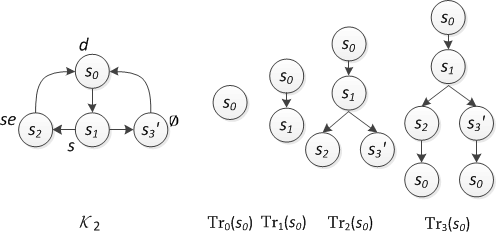
\includegraphics[width=10cm]{chapter05/NK2Tree1.png}
		\caption{左图为初始$\MPK$-结构$\mathcal{K}_2$ (源于图~\ref{Fig:chapter04:v1uv2}); 右图:从左到右表示以$s_0$为根、深度分别为0、1、2和3的计算树(为简化图,计算树的标签没有给出,但是每个树节点的标签可从${\cal K}_2$找到。)}\label{fig:K2Tree}
	\end{figure*}

%\begin{figure*}[!htb]
%	\centering
%	% Requires \usepackage{graphicx}
%	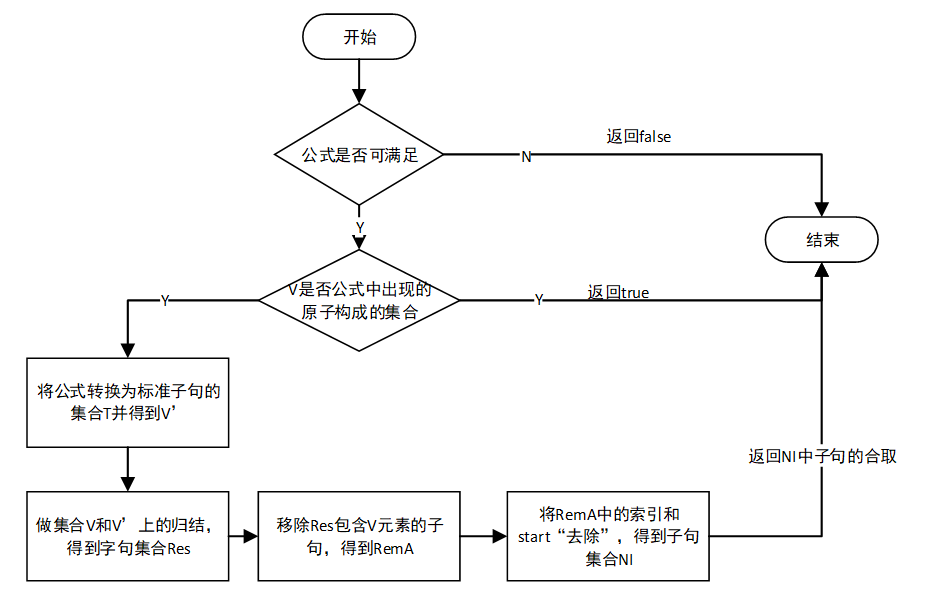
\includegraphics[width=15cm]{chapter04/frame.png}\\
%	\caption{基于归结的遗忘的主要流程图}
%	\label{Fig:chapter05:v1uv2}
%\end{figure*}

\end{example}


下面的定理表示上述定义的特征公式确实描述了一个初始\MPK-结构,此时对系统结构的操作就可转换为对其特征公式的操作,如下文将要讲的给定系统下的最弱充分条件计算。更直观地说,特征公式保持了给定初始$\MPK$-结构在原子命题集合$V$上的所有特性,即:具有$\overline{V}$-互模拟的两个初始$\MPK$-结构关于$V$的特征公式逻辑等价。

\begin{theorem}\label{CF}
	令$V\subseteq \Ha$、$\Hm=(S,R,L,s_0)$且$\Hm'=(S',R', L',s_0')$,则:
	\begin{itemize}
		\item[(i)] $(\Hm',s_0') \models {\cal F}_V({\cal M},s_0)
		\text{ 当且仅当 }
		({\cal M},s_0) \lrto_{\overline V} ({\cal M}',s_0')$;
		
		\item[(ii)] 若$s_0 \lrto_{\overline V} s_0'$则${\cal F}_V(\Hm, s_0) \equiv {\cal F}_V(\Hm', s_0')$。
	\end{itemize}
	
\end{theorem}
\begin{proof}
	(i) 令${\cal F}_V(\Hm, s_0)$为$(\Hm, s_0)$关于$V$的特征公式。显然,$\IR({\cal F}_V(\Hm, s_0), \overline V)$。为了证明上述结论成立,下面证明首先证明$(\Hm, s_0) \models {\cal F}_V(\Hm, s_0)$。
	
	令$c={ch({\cal M},V)}$,由引理~\ref{Bn:to:Tn}可知$(\Hm, s_0) \models {\cal F}_V(\Tr_c(s_0))$。下面证明特征公式里的另一部分,即:$(\Hm, s_0) \models \bigwedge_{s\in S} \ALL\GLOBAL\ G(\Hm, s)$,其中
	\[G(\Hm, s) = {\cal F}_V(\Tr_c(s)) \rto \left(\bigwedge_{(s,s_1) \in R} \EXIST \NEXT {\cal F}_V(\Tr_c(s_1))\right)\wedge \ALL \NEXT \left(\bigvee_{(s,s_1) \in R} {\cal F}_V(\Tr_c(s_1))\right).\]
	
	为此,下面证明$(\Hm, s_0) \models \ALL\GLOBAL\ G(\Hm, s)$。考虑下面两种情况:
	\begin{itemize}
		\item  若$(\Hm, s_0) \not \models {\cal F}_V(\Tr_c(s))$,显然$(\Hm, s_0) \models G(\Hm, s)$;
		\item 若$(\Hm, s_0) \models {\cal F}_V(\Tr_c(s))$:\\
		$(\Hm, s_0) \models {\cal F}_V(\Tr_c(s))$\\
		$\Rto$  $s_0 \lrto_{\overline V} s$ \hfill (引理~\ref{div_s})
		
		$\forall (s, s_1)\in R$:\\
		$(\Hm, s_1) \models {\cal F}_V(\Tr_c(s_1))$  \hfill  ($s_1 \lrto_{\overline V} s_1$)\\
		$\Rto$ $(\Hm, s) \models \bigwedge_{(s,s_1)\in R}\EXIST \NEXT {\cal F}_V(\Tr_c(s_1))$\\
		$\Rto$ $(\Hm, s_0) \models$ $\bigwedge_{(s,s_1)\in R}\EXIST \NEXT {\cal F}_V(\Tr_c(s_1))$    \qquad  ($\IR(\bigwedge_{(s,s_1)\in R}\EXIST \NEXT {\cal F}_V(\Tr_c(s_1)), \overline V)$, $s_0 \lrto_{\overline V} s$)
		
		$\forall (s, s_1) \in R$:\\
		$(\Hm, s_1) \models \bigvee_{(s, s_2)\in R}{\cal F}_V(\Tr_c(s_2))$\\
		$\Rto$ $(\Hm, s) \models \ALL \NEXT \left( \bigvee_{(s, s_2)\in R} {\cal F}_V(\Tr_c(s_2)) \right)$ \\
		$\Rto$ $(\Hm, s_0) \models$  $\ALL \NEXT \left( \bigvee_{(s, s_2)\in R} {\cal F}_V(\Tr_c(s_2)) \right)$   \hfill   ($\IR(\ALL \NEXT \left( \bigvee_{(s, s_2)\in R} {\cal F}_V(\Tr_c(s_2)) \right), \overline V)$, $s_0 \lrto_{\overline V} s$)\\
		$\Rto$ $(\Hm, s_0) \models G(\Hm, s)$。\\
		% where $s_i$ and $s_j$ are the successors of $s$.
	\end{itemize}
	
	对任意其他能从$s_0$可达的状态$s'$,都可以类似地证明$(\Hm,s')\models G(\Hm, s)$。
	因此,对任意的$s\in S$,$(\Hm, s_0) \models \ALL\GLOBAL\ G(\Hm, s)$,从而$(\Hm, s_0) \models {\cal F}_V(\Hm, s_0)$。
	
	下面从两个方面证明(i)成立:
	
	$(\Lto)$ 证明:若$s_0 \lrto_{\overline V} s_0'$,则$(\Hm',s_0') \models {\cal F}_V(M,s_0)$。因为$(\Hm, s_0) \models {\cal F}_V(\Hm, s_0)$且 $\IR({\cal F}_V(\Hm, s_0), \overline V)$,由定理~\ref{thm:V-bisimulation:EQ}可知
	$(\Hm',s_0') \models {\cal F}_V(M,s_0)$。
	
	$(\Rto)$ 证明:若$(\Hm',s_0') \models {\cal F}_V(M,s_0)$,则$s_0 \lrto_{\overline V} s_0'$。为此,下面证明对任意的$n \geq 0$,$Tr_n(s_0) \lrto_{\overline V} Tr_n(s_0')$。
	
	
	\textbf{基始($n=0$):} 由特征公式的定义,显然$Tr_0(s_0) \equiv Tr_0(s_0')$成立。
	
	\textbf{归纳步骤($n>0$):} 假定对任意的$k > 0$都有$\Tr_k(s_0) \lrto_{\overline V} \Tr_k(s_0')$,下面证明$\Tr_{k+1}(s_0) \lrto_{\overline V} \Tr_{k+1}(s_0')$。令$(s_0, s_1), (s_1, s_2)$, $\dots$, $(s_{k-1}, s_k) \in R$且$(s_0', s_1'), (s_1', s_2'), \dots, (s_{k-1}', s_k') \in R'$,即对于任意的$0 \leq i \leq k-1$,$s_{i+1}$($s_{i+1}'$)是$s_i$ ($s_i'$)的直接后继状态。
	由归纳假设可知,只需证明$\Tr_1(s_k) \lrto_{\overline V} \Tr_1(s_k')$。
	
	(a) 由归纳假设可知$L(s_k) - \overline V = L'(s_k') - \overline V$。
	
	在讨论其他点时,首先考虑下面事实(\textbf{fact}):\\
	$(\Hm',s_0') \models {\cal F}_V(\Hm,s_0)$\\
	$\Rto$ $\forall s'\in S'$,$\forall s\in S$,\\ $(\Hm', s')\models {\cal F}_V(\Tr_c(s)) \rto$  $\left(\bigwedge_{(s,s_1)\in R} \EXIST \NEXT {\cal F}_V(\Tr_c(s_1))\right)\wedge \ALL \NEXT \left( \bigvee_{(s,s_1)\in R} {\cal F}_V(\Tr_c(s_1))\right)$  \\
	(I) $(\Hm', s_0') \models {\cal F}_V(\Tr_c(s_0)) \rto \left(\bigwedge_{(s_0, s_1) \in R} \EXIST \NEXT {\cal F}_V(\Tr_c(s_1))\right)$ $\wedge$ $\ALL \NEXT \left(\bigvee_{(s_0, s_1) \in R} {\cal F}_V(\Tr_c(s_1)) \right)$     \\
	(II) $(\Hm', s_0') \models {\cal F}_V(\Tr_c(s_0)))$  \hfill  (已知)\\
	(III) $(\Hm', s_0') \models \left(\bigwedge_{(s_0, s_1) \in R} \EXIST \NEXT {\cal F}_V(\Tr_c(s_1))\right)$ $\wedge$ $\ALL \NEXT \left(\bigvee_{(s_0, s_1) \in R} {\cal F}_V(\Tr_c(s_1)) \right)$  \hfill  ((I),(II))\\
	
	% It is apparent that $L'(s_0') - \overline V = L(s_0) - \overline V$;\\
	(b) 这里证明$\forall (s_k, s_{k+1}) \in R$,存在$(s_k', s_{k+1}') \in R'$使得$L(s_{k+1}) - \overline V = L'(s_{k+1}') - \overline V$。\\
	(1) $(\Hm', s_0') \models \bigwedge_{(s_0, s_1) \in R} \EXIST \NEXT {\cal F}_V(\Tr_c(s_1))$  \hfill  (III)\\
	(2) $\forall (s_0, s_1) \in R$,$\exists (s_0', s_1') \in R'$ 使得 $(\Hm', s_1') \models {\cal F}_V(\Tr_c(s_1))$  \hfill  (1)\\
	(3) $\Tr_c(s_1) \lrto_{\overline V} \Tr_c(s_1')$  \hfill  ((2), 引理~\ref{Bn:to:Tn}) \\
	(4) $L(s_1) - \overline V = L'(s_1') - \overline V$  \hfill   ((3), $c \geq 0)$\\
	(5) $(\Hm', s_1') \models {\cal F}_V(\Tr_c(s_1)) \rto \left(\bigwedge_{(s_1,s_2)\in R} \EXIST \NEXT {\cal F}_V(\Tr_c(s_2))\right) \wedge \ALL \NEXT \left(\bigvee_{(s_1,s_2)\in R} {\cal F}_V(\Tr_c(s_2))\right)$     \hfill  \textbf{(fact)}\\
	(6) $(\Hm', s_1') \models \left(\bigwedge_{(s_1,s_2)\in R} \EXIST \NEXT {\cal F}_V(\Tr_c(s_2))\right) \wedge \ALL \NEXT \left(\bigvee_{(s_1,s_2)\in R} {\cal F}_V(\Tr_c(s_2))\right)$ \hfill ((2), (5))\\
	(7) $\dots \dots$ \\
	(8) $(\Hm', s_k') \models \left(\bigwedge_{(s_k,s_{k+1})\in R} \EXIST \NEXT {\cal F}_V(\Tr_c(s_{k+1}))\right) \wedge \ALL \NEXT \left(\bigvee_{(s_k,s_{k+1})\in R} {\cal F}_V(\Tr_c(s_{k+1}))\right)$       \hfill (与(6)类似)\\
	(9) $\forall (s_k, s_{k+1}) \in R$,$\exists (s_k', s_{k+1}') \in R'$ 使得$(\Hm', s_{k+1}') \models {\cal F}_V(\Tr_c(s_{k+1}))$  \hfill  (8)\\
	(10) $\Tr_c(s_{k+1}) \lrto_{\overline V} \Tr_c(s_{k+1}')$    \hfill ((9), 引理~\ref{Bn:to:Tn}) \\
	(11) $L(s_{k+1}) - \overline V = L'(s_{k+1}') - \overline V$  \hfill   ((10), $c \geq 0)$\\
	
	(c) 这里证明$\forall (s_k', s_{k+1}') \in R'$,存在$(s_k, s_{k+1})\in R$ 使得$L(s_{k+1}) - \overline V = L'(s_{k+1}') - \overline V$。\\
	(1) $(\Hm', s_k') \models \ALL \NEXT \left(\bigvee_{(s_k,s_{k+1})\in R} {\cal F}_V(\Tr_c(s_{k+1}))\right)$  \hfill (上面的(8))\\
	(2) $\forall (s_k', s_{k+1}') \in R'$,$\exists (s_k, s_{k+1}) \in R$ 使得$(\Hm', s_{k+1}') \models {\cal F}_V(\Tr_c(s_{k+1}'))$  \hfill (1) \\
	(3) $\Tr_c(s_{k+1}) \lrto_{\overline V} \Tr_c(s_{k+1}')$    \hfill ((2), 引理~\ref{Bn:to:Tn}) \\
	(4) $L(s_{k+1}) - \overline V = L'(s_{k+1}') - \overline V$  \hfill   ((3), $c \geq 0)$\\
	
	(ii) 由引理~\ref{lem:Vb:TrFormula:Equ}和\ref{div_s}易知。
	
\end{proof}

\section{遗忘理论的封闭性及复杂性结果}\label{chapter06:sec:close}
当给定的$\CTL$公式的长度(字符的个数)为$n$,由小模型理论可知定义在状态个数为$k=n8^n$的状态空间${\cal S}=\{s_1,s_2,\dots, s_k\}$上的初始结构就能保证公式的可满足性~\cite{DBLP:journals/jcss/EmersonH85}。
对于其他拥有同样大小的状态空间上的任意初始$\MPK$-结构,都能在${\cal S}$状态空间上找到一个初始$\MPK$-结构与之互模拟,且由定理~\ref{CF}可知他们有相同的特征公式。
因此,只有有限个初始$\MPK$-结构作为该公式的候选模型。因此下面结论成立。
%这一事实可以用下面引理表示。

\begin{lemma}\label{lem:models:formula}
	给定$\CTL$公式$\varphi$,下面等式成立:
	\begin{equation*}
		\varphi\equiv \bigvee_{(\Hm, s_0)\in\Mod(\varphi)}{\cal F}_{\cal A}(\Hm, s_0).
	\end{equation*}
\end{lemma}
\begin{proof}
	令$(\Hm', s_0')$为$\varphi$的模型。由定理~\ref{CF}可知$(\Hm', s_0') \models {\cal F}_{\Ha}(\Hm', s_0')$,则:
	$$(\Hm', s_0') \models \bigvee_{(\Hm, s_0)\in \Mod(\varphi)} {\cal F}_{\Ha}(\Hm, s_0).$$
	
	另一方面,假定$(\Hm', s_0')$为$\bigvee_{(\Hm, s_0)\in \Mod(\varphi)} {\cal F}_{\Ha}(\Hm, s_0)$的模型。则存在$(\Hm, s_0)\in \Mod(\varphi)$使得 $(\Hm', s_0') \models {\cal F}_{\Ha}(\Hm,$ $s_0)$。由定理~\ref{CF}可知$(\Hm, s_0) \lrto_{\emptyset} (\Hm', s_0')$,从而由定理~\ref{thm:V-bisimulation:EQ}可知$(\Hm, s_0)$ 是 $\varphi$的一个模型。
\end{proof}

这一结论表明:任意的$\CTL$公式都与其模型的特征公式的吸取逻辑等价。这对遗忘理论的封闭性提供了重要的理论支撑,也即是从公式里遗忘掉原子命题集合$V$中的元素只需找到与给定公式的模型$V$-互模拟的那些模型就能确定遗忘的结果。形式化地,对于给定的公式$\varphi$和原子命题集合$V$,从$\varphi$中遗忘掉$V$中的元素得到的结果为:
\begin{equation*}
	\bigvee_{{\cal K}\in  \{{\cal K}'\mid \exists {\cal K}''\in\Mod(\phi)\ \text{ and }\ {\cal K}''\lrto_V{\cal K}'\}} {\cal F}_{\overline V}({\cal K}).
\end{equation*}



下面分析遗忘在$\CTL$段$\CTL_{\ALL\FUTURE}$下各种任务的复杂性结果,其中$\CTL_{\ALL\FUTURE}$表示$\CTL$公式只包含时序算子$\ALL \FUTURE$的子类。
这一类公式在并发系统中的互斥和等待等属性描述中有重要作用~\cite{Baier:PMC:2008},尽管这类公式是相对简单的,但是下面将要说明判定一个模型是否为从此类公式中遗忘掉原子命题集合得到的结果的模型是$\textsc{NP}$-完全的。
\begin{proposition}[模型检测]
	\label{modelChecking}
	给定一个结构 $(\Hm,s_0)$、原子命题集合$V\subseteq{\cal A}$ 和公式 $\varphi \in \CTL_{\ALL\FUTURE}$,判定 $(\Hm,s_0) \models^? \CTLforget(\varphi, V)$ 是 \textsc{NP}-完全的。
\end{proposition}
\begin{proof}
	成员属性(Membership). 假定$(\Hm,s_0) \models \CTLforget(\varphi,V)$,则存在一个初始结构$(\Hm', s_0')$ 使得 (a) $(\Hm',s_0') \models \varphi$ 且 (b) $(\Hm,s_0) \lrto_V (\Hm',s_0')$。已有结果表明,(a) 能在$\Hm'$ 和 $\varphi$ 的大小的多项式时间内完成~\cite{DBLP:books/daglib/0007403}。条件(b) 也可用Baier等人的推论推论 7.45~\cite{Baier:PMC:2008}的方法证明能在多项式时间内完成。
	又因为猜$(\Hm,s_0)$多项式大小的初始结构$(\Hm',s_0')$能在多项式时间内完成,因此,这一问题在$\textsc{NP}$ 中。
	
	困难属性(Hardness). 已经证明命题逻辑下遗忘的模型检测是$\textsc{NP}$-难的,由于命题逻辑下的遗忘是$\CTL$的一种~\cite{Zhang2008Properties}。因此,上述问题是$\textsc{NP}$-难的。
\end{proof}

关于遗忘的逻辑蕴涵问题也是值得考虑的,下面讨论$\CTL_{\ALL\FUTURE}$段下关于遗忘的逻辑蕴涵的复杂性。

\begin{theorem}[Entailment]
	\label{thm:comF}
	令 $\varphi$ 和 $\psi$ 为$\CTL_{\ALL \FUTURE}$中的两个公式, $V$ 为原子命题的集合。则:
	\begin{itemize}
		\item[(i)] 判定  $\CTLforget(\varphi, V ) \models^? \psi$ 是 co-$\textsc{NP}$-完全的,
		\item[(ii)] 判定  $\psi \models^? \CTLforget(\varphi, V)$ 是 $\Pi_2^{\textsc{P}}$-完全的,
		\item[(iii)] 判定 $\CTLforget(\varphi, V) \models^? \CTLforget(\psi, V)$ 是 $\Pi_2^{\textsc{P}}$-完全的。
	\end{itemize}
\end{theorem}
\begin{proof}
	(i) 困难属性. 已有结论表明,判定公式$\varphi$是否是可满足的是$\textsc{NP}$-完全的~\cite{meier2009complexity}。要整困难属性,通过令$\CTLforget(\varphi, V)\equiv \top$,只需证明$\psi$是有效的,即:原问题是co-NP-难的。
	
	成员属性. 定理~\ref{thm:exist} 表明$\CTLforget(\varphi, V) \models \psi$ 当且仅当 $\varphi \models \psi$ 且 $\IR(\psi, V)$。
	在$\CTL_{\ALL \FUTURE}$ 中,判定 $\varphi \models \psi$ 是co-$\textsc{NP}$ 的~\cite{meier2009complexity}。
	这里证明 $\IR(\psi, V)$ 是否成立是 co-$\textsc{NP}$ 的。不失一般性地,假定$\psi$ 是可满足的,则 $\psi$ 有一个大小为$|\psi$的多项式的模型。
	这里讨论该问题的补问题:判定 $\psi$ 是$V$-有关的,即 $\neg \IR(\psi, V)$。显然,$\neg \IR(\psi, V)$ 当且仅当存在$\psi$的一个模型 $(\Hm,s_0)$ 和大小为$|\psi|$的多项式的初始结构 $(\Hm',s_0')$ 使得 $(\Hm,s_0) \lrto_V (\Hm',s_0')$ 且 $(\Hm',s_0') \not \models \psi$。因此,判定$\neg \IR(\psi, V)$是否成立有如下两个步骤:(1) 猜两个大小为$|\psi|$的多项式的初始结构$(\Hm,s_0)$ 和 $(\Hm',s_0')$ 使得 $(\Hm,s_0) \models \psi$ 且 $(\Hm',s_0') \not \models \psi$,和 (2)
	检查 $(\Hm,s_0) \lrto_V (\Hm',s_0')$。
	显然, (1) 和(2) 都是能在多项式时间内完成的。
	
	(ii) 成员属性. 考虑这一问题的补问题。猜一个大小为$\psi$ 的多项式的$\psi$ 的 模型 $(\Hm,s_0)$ 且检查 是否 $(\Hm, s_0) \not \models \CTLforget(\varphi, V)$。
	由命题~\ref{modelChecking} 可知这一问题在 $\Sigma_2^{\textsc{P}}$中。因此,原问题在$\Pi_2^{\textsc{P}}$中。
	
	困难属性. 令$\psi \equiv \top$。 则这一问题被规约为判定$\CTLforget(\varphi, V)$的有效性问题。 
	由于命题遗忘是$\CTL$遗忘的特殊情形,因此该问题的困难属性直接来源于\cite{DBLP:journals/jair/LangLM03}。

(iii) 成员属性. 假定 $\CTLforget(\varphi, V) \not \models \CTLforget(\psi, V)$。则存在一个初始结构 $(\Hm,s) 
\models \CTLforget(\varphi, V)$ 且$(\Hm,s) \not \models \CTLforget(\psi, V)$,即存在一个初始结构$(\Hm_1,s_1) \lrto_V (\Hm,s)$ 使得 $(\Hm_1, s_1) \models \varphi$ 但是对其他$(\Hm, s) \lrto_V (\Hm_2,s_2)$ 使得 $(\Hm_2, s_2) \not \models \psi$。
由命题~\ref{modelChecking} 的证明可知,$(\Hm,s)$和 $(\Hm_1,s_1)$ 能在$|\varphi|$、$|\psi|$和$|V|$的多项式时间内完成。 
显然,猜使得$(\Hm_1,s_1) \lrto_V (\Hm,s)$ 成立的大小为$|\varphi$多项式的 $(\Hm,s)$和 $(\Hm_1,s_1)$ 可以在多项式时间内完成,且 对任意的 $(\Hm, s) \lrto_V (\Hm_2,s_2)$,检查 $(\Hm_2,s_2) \not \models \psi$ 可以在 $|\psi|$ 和 $|\Hm_2|$ 的多项式时间内完成。
因此,该问题是 $\Pi_2^{\textsc{P}}$的。

困难属性. 由于 $\IR(\CTLforget(\psi, V), V) $,因此 $\CTLforget(\varphi, V) \models \CTLforget(\psi, V)$ 当且仅当 $\varphi \models \CTLforget(\psi, V)$。 所以由(ii)不难证明该问题。
\end{proof}



定理~\ref{thm:comF}蕴涵下列结论。
\begin{corollary}
	令 $\varphi$ 和 $\psi$ 为 $\CTL_{\ALL \FUTURE}$中的两个公式,$V$原子公式的集合。则
	\begin{itemize}
		\item[(i)] 判定 $\psi \equiv^?\CTLforget(\varphi, V)$ 是 $\Pi_2^{\textsc{P}}$-完全的,
		\item[(ii)] 判定 $\CTLforget(\varphi, V) \equiv^? \varphi$ 是 co-$\textsc{NP}$-完全的,
		\item[(iii)] 判定 $\CTLforget(\varphi, V) \equiv^? \CTLforget(\psi, V)$ 是$\Pi_2^{\textsc{P}}$-完全的。
	\end{itemize}
\end{corollary}

%在上述的遗忘理论的定义中说明了如果公式$\psi$的任意一个模型${\cal K}$都能找到$\varphi$的一个模型${\cal K}'$使得${\cal K} \lrto_V {\cal K}'$,则称$\psi$为从$\varphi$中遗忘掉$V$中原子命题后得到的结果。为刻画S5逻辑下该概念的直观含义,Zhang等人提出了如下遗忘理论特性——这些特性被称为\emph{遗忘理论公设}(forgetting postulates)~\cite{Yan:AIJ:2009}。
%给定$\CTL$公式$\varphi$、$\varphi'=\CTLforget(\varphi, V)$和原子命题集合$V\subseteq \Ha$和$\varphi'=\CTLforget(\varphi, V)$,遗忘理论公设如下:
%\begin{itemize}
%	\item[] (\W) 弱(Weakening)属性:$\varphi \models \varphi'$;
%	\item[] (\PP) 正支持性(Positive Persistence):对任意与$V$无关的公式$\eta$,若$\varphi \models \eta$则$\varphi' \models \eta$;
%	\item[] (\NgP) 负支持性(Negative Persistence):对任意与$V$无关的公式$\eta$,若$\varphi \not \models \eta$则$\varphi' \not \models \eta$;
%	\item[] (\textbf{IR}) 无关性(Irrelevance): $\IR(\varphi', V)$
%\end{itemize}
%直观地说,(\W)和(\textbf{IR})表明“遗忘”削弱了公式$\varphi$且得到的结果与$V$无关,(\PP)和(\NgP)表明对任意与$V$无关的公式$\eta$,$\varphi \models \eta$当且仅当$\varphi' \models \eta$。总而言之,遗忘得到的结果能推出所有与$V$无关且能被$\varphi$推出的结果,且不能推出所有与$V$无关且不能被$\varphi$推出的结果。
%从数据库和安全的层面讲,遗忘相当于从已有的关系表中构建出一个视图,达到了隐私保护的作用。
%下面的定理表明$\CTL$中的遗忘理论与上述公设也具有当且仅当的关系。
%
%\begin{theorem}[Representation Theorem]\label{thm:close}
%	%Let $\varphi$, $\varphi'$ and $\phi$ be \CTL\
%	给定$\CTL$公式$\varphi$和$\varphi'$,$V \subseteq \Ha$为原子命题的集合。
%	%Then t
%	下面的陈述是等价的:
%	\begin{itemize}
%		\item[(i)] $\varphi' \equiv \CTLforget(\varphi, V)$,
%		\item[(ii)] $\varphi'\equiv \{\phi \mid\varphi \models \phi \text{ and } \IR(\phi, V)\}$,
%		\item[(iii)] 若$\varphi$、$\varphi'$和$V$为(i)和(ii)中提到的符号,则公设(\W)、(\PP)、(\NgP)和(\textbf{IR})成立. 
%	\end{itemize}
%\end{theorem}
%\begin{proof}
%	$(i) \LRto (ii)$. 为了证明这个结论,只需证明如下等式成立:
%	\[
%	\Mod(\CTLforget(\varphi, V)) = \Mod(\{\phi \mid \varphi \models \phi, \IR(\phi, V)\}).\]
%	$(\Rto)$ 对任意$\CTLforget(\varphi, V)$的模型${\cal K}'$ \\
%	$\Rto$  $\exists {\cal K}$使得${\cal K} \models \varphi$且${\cal K} \lrto_V {\cal K}'$ \hfill (定义~\ref{def:V:forgetting}) \\
%	$\Rto$ $\forall \phi$,若$\varphi \models \phi$且$\IR(\phi, V)$则${\cal K}' \models \phi$  \hfill (定理~\ref{thm:V-bisimulation:EQ})\\
%	$\Rto$ ${\cal K}' \models \{\phi \mid \varphi \models \phi, \IR(\phi, V)\}$
%	
%	$(\Lto)$ 因为$\IR(\CTLforget(\varphi, V),V)$且$\varphi \models \CTLforget(\varphi, V)$,由定义~\ref{def:V:forgetting}可知$\{\phi \mid \varphi \models \phi, \IR(\phi, V)\} \models \CTLforget(\varphi, V)$。
%	
%	$(ii) \Rto (iii)$.令$A = \{\phi \mid \varphi \models \phi, \IR(\phi, V)\}$。 
%	首先,由于对任意的$\phi'\in A$都有$\varphi \models \phi'$,所以$\varphi \models \varphi'$。
%	其次,对任意的公式$\phi$,若$\IR(\phi, V)$且$\varphi \models \phi$则$\phi \in A$,因此$\varphi' \models \phi$.
%	第三, 对任意的公式$\phi$,若$\IR(\phi, V)$且$\varphi \not \models \phi$则$\phi \not \in A$。因此$\varphi' \not \models \phi$。
%	最后,因为对任意的$\phi' \in A$都有$\IR(\varphi',V)$ ,所以$\IR(\phi',V)$。
%	
%	$(iii) \Rto (ii)$.一方面,由(\PP) 和 (\NgP)可知,对任意的公式$\phi'$且$\IR(\phi',V)$,$\varphi \models \phi'$当且仅当$\varphi' \models \phi'$。所以对任意的$\phi'\in \{\phi \mid \varphi \models \phi, \IR(\phi, V)\}$都有$\varphi' \models \phi'$,因而$\varphi' \models \{\phi \mid \varphi \models \phi, \IR(\phi, V)\}$。 
%	另一方面,由 (\W) 和 (\textbf{IR})可知$\{\phi \mid \varphi \models \phi, \IR(\phi, V)\} \models \varphi'$。因此,$\varphi'\equiv \{\phi \mid\varphi \models \phi \text{ and } \IR(\phi, V)\}$。
%\end{proof}


\section{基于模型的遗忘理论计算方法}\label{chapter06:sec:algm}
前几节中讲述的过程显然给出了一种计算遗忘的方法,本届将这些过程组织起来构成一个算法。该算法与第\ref{cha4:sec:alg}节中基于语法的算法不同,它是一种基于模型的算法(算法~\ref{alg:compute:forgetting:by:VB}),也就是说本节的算法通过计算所有可能的模型来计算遗忘,且其正确性可由引理\ref{lem:models:formula}和定理\ref{CF}保证。


\begin{algorithm}[tb]
	\caption{\small A Model-based \CTL\ Forgetting Procedure}
	\label{alg:compute:forgetting:by:VB}
	\LinesNumbered
	\KwIn{A \CTL formula $\varphi$ and a set $V$ of atoms}
	\KwOut{$\CTLforget(\varphi, V)$}% ????
	$\psi \lto \bot$\;
	\ForEach{initial \MPK-structure $\cal K$ (over $\cal A$ and $\cal S$)}{
		\lIf{${\cal K}\not\models\varphi$}{{\bf continue}} \\
		\ForEach{initial \MPK-structure ${\cal K}'$ with ${\cal K}\lrto_{ V}{\cal K}'$}{
			$\psi \lto \psi \lor {\cal F}_{\overline V}({\cal K}')$\;
		}
	}
	\Return $\psi$\;
\end{algorithm}



下面的例子来源于研究背景和意义部分,这里给出如何计算从规范中遗忘掉一些原子命题。 
\begin{example}\label{ex:6}
	对于图\ref{BVM}中的 ${\cal K}_1$,假定一个已知的规范(性质)为$\alpha = \EXIST\FUTURE(se \wedge sp)$。显然 ${\cal K}_1$满足 $\alpha$。若想移除掉 $sp$,即从 $\alpha$中遗忘掉 $sp$ ,则 $\CTLforget(\alpha,\{ sp\}) \equiv \EXIST\FUTURE se$。此时,该汽车制造公司可以用新的规范$\EXIST\FUTURE se$(这保证驾车最终会被生产)引导未来汽车的生产。
\end{example}


正如下面命题展示的那样,通过计算所有可能的模型是非常低效的,但是这为从理论的角度探索遗忘有重要作用。


\begin{proposition}\label{pro:time:alg1}
	令 $\varphi$ 为$\CTL$公式,$V\subseteq \Ha$为原子命题集合,状态空间的大小为 $|{\cal S}|=m$, $|\Ha|=n$ 和 $|V|=x$。则使用算法\ref{alg:compute:forgetting:by:VB}计算从$\varphi$中遗忘掉$V$中原子的空间复杂度为 $O((n-x)m^{2(m+2)}2^{nm}  \log m)$,且时间复杂性至少与空间复杂性相同。
\end{proposition}
\begin{proof}
假定每个状态或原子命题占据$\log m$的空间且$n\leq m$,则一个状态对$(s,s')$占据$2*\log m$位(bit)。对任意的$B \subseteq {\cal S}$ 且$s_0\in B$,构造如下初始结构$(\Hm,s_0)$,其中$\Hm = (B,R,L,s_0)$,则$R$中至多有$\frac{|B|^2}{2}$个状态对且$L$中至多$|B|*n$个$(s,A)$对($A\subseteq \Ha$)。因此,$(\Hm,s_0)$至多占据$(|B|+|B|^2+|B|*n)*\log m$位。此外,对于状态集合$B$,初始状态有$|B|$种选择,有$|B|^{|B|}$种关系$R$,$(2^n)^{|B|}$种标签函数$L$。

在最坏的情形下(即$|B|=m$),可由构成$m * (m^m * 2^{nm} * m)$个初始结构。因此,最多有$m^{m+2} * 2^{nm}$个初始结构,且最多花费$(m^{m+2} * 2^{nm} * (m + m^2 + nm))* \log m$位。

令 $k = n-x$,对任意有$i\geq 1$个状态的初始结构${\cal K} = (\Hm,s_0)$,其中$\Hm = (B,R,L,s_0)$。
在最坏的情形下(即$ch(\Hm,V) = i$时),可以花费$N(i) = P_i(s_0) + i * (P_i(s) + i *P_i(s'))$位来存储${\cal K}$在$\overline{V}$上的特征公式。
其中$s',s\in B$,$P_i(y)$是存储${\cal F}_{\overline{V}}(\Tr_i(y))$($y\in B$)所用的空间(这里假定$\EXIST\NEXT$和$\ALL\NEXT$使用了相同的存储单位)。

${\cal F}_{\overline{V}}(\Tr_i(y))$ ($0\leq n \leq i$)被递归地定义如下:
\begin{align*}
	&(1) n=0,  \qquad P_0(y) = k\\
	&(2) n=1, \qquad  P_1(y) = k + i*k = k + i*P_0(y)\\
	&(3) n=2, \qquad P_2(y) = k + i*(k + i*k) = k+i*P_1(y)\\
	& \dots \qquad \qquad \dots\\
	&(i+1) n = i, \quad P_i(y) = k + i * P_{i-1}(y).
\end{align*}

因此,有
\begin{align*}
	P_i(y) & = k + i*k + i^2 * k + \dots + i^i * k = \frac{i^i -1}{i-1} k,\\
	N(i) & = P_i(s_0) + i* (P_i(s) + i * P_i(s'))\\
	& = (i^2 + i +1) P_i(y) \\
	& = (i^2 + i+1)\frac{i^i -1}{i-1} k.
\end{align*}
	
在最坏的情形下(即具有$m$个状态的初始结构)有$m^{m+2} * 2^{nm}$初始结构,需要$(m^{m+2} * 2^{nm} * N(m)) * \log m$位来存储遗忘的结果。

因此,空间复杂性为$O((n-x)m^{2(m+2)}2^{nm}* \log m)$。
\end{proof}


\section{本章小结}\label{sec:chapter05-conclusion}
本章讨论了一种基于模型的计算约束$\CTL$下遗忘的计算。为此,本章第一节首先提出了一种约束$V$-互模拟概念,并证明了该约束$V$-互模拟与$V$-互模拟在有限结构下是等价的。此外,定义了给定深度的计算树在给定原子命题集合上的特征公式,由此定义了有限结构的特征公式。结论表明初始结构能够满足给定的特征公式当且仅当该初始结构与特征公式对应的初始结构在给定原子命题集合上互模拟。基于此,得出了任意公式语义等价于其所有模型的特征公式的吸取,因为可以计算遗忘的结果。最后,本章给出了基于模型的计算遗忘的算法,并分析该算法关于公式的大小是指数空间的。

